\documentclass[169]{beamer}

\usepackage{listings}
\usepackage{listings-rust}

\usetheme{metropolis}

\title{An Overview of the Embedded Rust Ecosystem}
\subtitle{Or, Why are there so many crates, and what do they do?}
\author{Frans Skarman aka. TheZoq2}


% \usepackage{fontspec}
% \setmonofont[Contextuals={Alternate}]{Hasklug Nerd Font}

\definecolor{mygreen}{rgb}{0,0.6,0}
\definecolor{mygray}{rgb}{0.5,0.5,0.5}
\definecolor{mymauve}{rgb}{0.58,0,0.82}
\lstset{ 
    % choose the background color; you must add \usepackage{color} or \usepackage{xcolor}; should come as last argument
    % backgroundcolor=\color{white},
    % the size of the fonts that are used for the code
    basicstyle=\small\ttfamily,
    % sets if automatic breaks should only happen at whitespace
    breakatwhitespace=false,
    % sets automatic line breaking
    breaklines=true,
    % comment style
    commentstyle=\color{mygreen},
    % if you want to delete keywords from the given language
    deletekeywords={...},
    % if you want to add LaTeX within your code
    escapeinside={\%*}{*)},
    % lets you use non-ASCII characters; for 8-bits encodings only, does not work with UTF-8
    extendedchars=true,
    % keeps spaces in text, useful for keeping indentation of code (possibly needs columns=flexible)
    keepspaces=true,
    % keyword style
    keywordstyle=\color{blue},
    % where to put the line-numbers; possible values are (none, left, right)
    numbers=none,
    % how far the line-numbers are from the code
    numbersep=5pt,
    % the style that is used for the line-numbers
    %numberstyle=\ttfamily\footnotesize\color{mygray},
    % if not set, the frame-color may be changed on line-breaks within not-black text (e.g. comments (green here))
    rulecolor=\color{black},
    % show spaces everywhere adding particular underscores; it overrides 'showstringspaces'
    showspaces=false,
    % underline spaces within strings only
    showstringspaces=false,
    % show tabs within strings adding particular underscores
    showtabs=false,
    % the step between two line-numbers. If it's 1, each line will be numbered
    stepnumber=1,
    % string literal style
    stringstyle=\color{mymauve},
    % sets default tabsize to 2 spaces
    tabsize=2,
    % show the filename of files included with \lstinputlisting; also try caption instead of title
}


\begin{document}
\maketitle

\begin{frame}
    \frametitle{Who am I?}
    
    Frans Skarman (@TheZoq2)

    \begin{itemize}
        \item Rust evangelist
        \item Maintainer of \texttt{stm32f1xx\_hal}
        \item My desk is covered in rust
    \end{itemize}
\end{frame}

\begin{frame}
    \frametitle{Who are you?}

    \begin{itemize}
        \item Embedded rust (this talk probably won't be very interesting for you)
        \item Arduino
        \item Embedded C
        \item Rust user
    \end{itemize}
\end{frame}

\begin{frame}
    \frametitle{Goals}

    There are lots of embedded crates

    How do they all fit together?

    Explained through showing the need for them
\end{frame}

\begin{frame}
    \frametitle{The lowest level}

    \begin{itemize}
        \item Micro controllers control I/O through ``registers''
        \item Typically memory mapped
        \item Read the datasheet for instructions
    \end{itemize}
\end{frame}

\begin{frame}{An example: turning on an LED}
    After reading the 12 pages about the GPIO peripheral
    \begin{itemize}
        \item{Power up the GPIO peripheral in the RCC register}
        \item{Configure pin as output}
        \item{In the correct mode}
        \item{Set output to High}
    \end{itemize}
\end{frame}

\begin{frame}{An example: turning on an LED}
    \begin{columns}
        \begin{column}{0.5\textwidth}
            Configure pin 5 as output

            \begin{itemize}
                \item{Registers are at offset \texttt{0x00}}
                \item{Offset from start of GPIOx}
                \item{Write \texttt{0b10} in bit 20, 21}
                \item{Write \texttt{0b01} in bit 23, 22}
            \end{itemize}

            Same deal for the output value.
        \end{column}
        \begin{column}{0.5\textwidth}
            \begin{figure}
                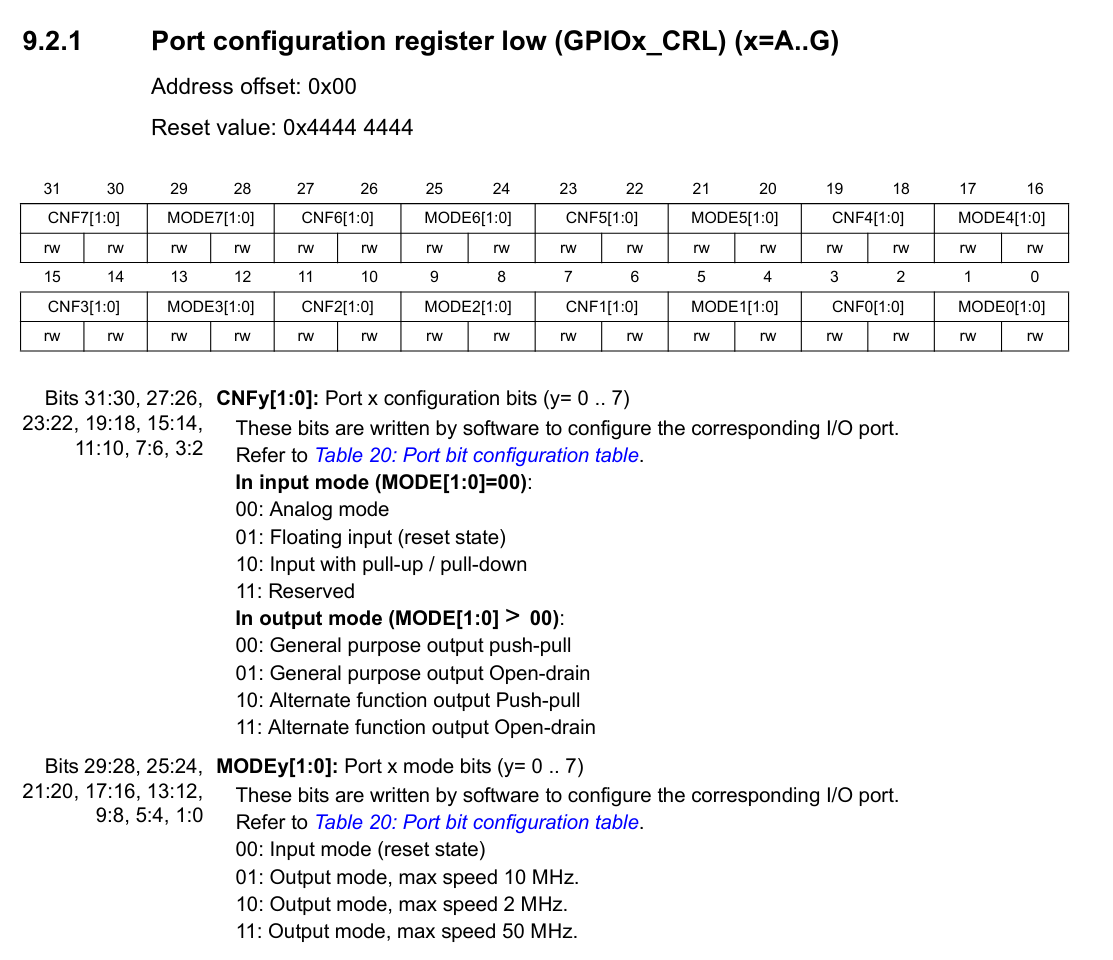
\includegraphics[width=\textwidth]{fig/gpio_crl.png}
            \end{figure}
        \end{column}
    \end{columns}
\end{frame}

\begin{frame}{The rust code}
    \begin{itemize}
        \item Very unsafe
        \item Very unergonomic
    \end{itemize}
\end{frame}

\begin{frame}{SVD files}
    \begin{itemize}
        \item{Published by microcontroller manufacturers}
        \item{Describes the function of each register}
        \item{\texttt{svd2rust} generates rust crates}
        \item{Usually have some errors that need manual intervention}
    \end{itemize}
\end{frame}

\begin{frame}{Peripheral Access Crates}
    \begin{itemize}
        \item{Result of patches + \texttt{svd2rust}}
        \item{\textit{Mostly} safe interface}
        \item{Adds a lot of zero cost abstraction (in release mode)}
        \item{Prevents re-use of peripherals}
        \item{TODO: Code example}
    \end{itemize}
\end{frame}

\begin{frame}{Peripheral Access Crates (PACs)}
    Fixed the unsafety and unclear code.

    But has some remaining issues

    \begin{itemize}
        \item{No check for peripheral dependencies}
        \item{Or correct intialisation}
        \item{=> Still requires through reading of the datasheet}
    \end{itemize}
\end{frame}

\begin{frame}[fragile]{Hardware Abstraction Layers (HALs)}
    A high level interface around the PAC

    \lstset{language=rust}
    \begin{lstlisting}
    // Set up common structs
    let mut rcc = dp.RCC.constrain();
    let clocks = rcc.cfgr.freeze(&mut flash.acr);

    // Acquire and configure the GPIOC peripheral
    let mut gpioc = dp.GPIOC.split(&mut rcc.apb2);

    // Set the pin mode
    let mut led = gpioc.pc13.into_push_pull_output(&mut gpioc.crh);
    // Turn the led on
    led.set_high()
    \end{lstlisting}
\end{frame}

\end{document}
